\documentclass[11pt,a4paper]{article}
\usepackage[T1]{fontenc}
\usepackage[utf8]{inputenc}
\usepackage{lmodern}
\usepackage{amsmath,amssymb,amsthm,mathtools,mathrsfs}
\usepackage{graphicx,float,xcolor,multicol}
\usepackage[shortlabels]{enumitem}
\usepackage[margin=27mm]{geometry}
\usepackage{microtype,needspace,placeins}
\usepackage{tikz,tikz-cd}
\usetikzlibrary{arrows.meta,calc,positioning,patterns,decorations.pathreplacing}
\usepackage[colorlinks=true,linkcolor=teal,urlcolor=teal,citecolor=teal]{hyperref}
\setlength{\parindent}{0pt}
\setlength{\parskip}{.6em}
\setcounter{secnumdepth}{0}
\allowdisplaybreaks
\raggedbottom
\providecommand{\cross}{\times}
\DeclareUnicodeCharacter{2020}{\ensuremath{\dagger}}
\DeclareMathOperator{\supp}{supp}
\DeclareMathOperator*{\esssup}{ess\,sup}
\providecommand{\chapter}{\section}
\newenvironment{tool}[2]{\subsection*{Tool #1 --- #2}}{}
\newcommand{\ToolRef}[1]{Tool #1}
\newcommand{\FigureTag}[2]{\textit{Figure #1}}
\newcommand{\Result}[1]{\subsection*{#1}}
\newcommand{\Application}[1]{\subsubsection*{Application\if\relax\detokenize{#1}\relax\else\space--- #1\fi}}
\newcommand{\ProofHeading}{\par\textit{Proof.}\space}
\newcommand{\ProofOf}[1]{\par\textit{Proof of #1.}\space}
\newcommand{\RemarkHeading}{\par\textbf{Remark.}\space}
\newcommand{\NoteHeading}{\par\textbf{Note.}\space}
\newcommand{\ExerciseHeading}{\par\textbf{Exercise.}\space}

% Rendering support only; mathematical text is in each independent post.
\usepackage{booktabs,array,longtable}
\definecolor{HandoutBlue}{HTML}{2F6690}
\definecolor{HandoutNavy}{HTML}{17365D}
\newtheorem{theorem}{Theorem}
\newtheorem{lemma}[theorem]{Lemma}
\newtheorem{proposition}[theorem]{Proposition}
\newtheorem{corollary}[theorem]{Corollary}
\newtheorem{conjecture}[theorem]{Conjecture}
\newtheorem{definition}{Definition}
\newtheorem{example}{Example}
\newtheorem{namedtoolcounter}{Tool}
\newenvironment{namedtool}[1]{\begin{namedtoolcounter}[#1]}{\end{namedtoolcounter}}
\newtheorem*{claim}{Claim}
\newtheorem*{remark}{Remark}
\newtheorem*{exercise}{Exercise}
\newtheorem*{question}{Question}
\newtheorem*{observation}{Observation}
\newcommand{\SourceChapter}[2]{\section*{#2}}
\newcommand{\Lecture}[2]{\section*{Lecture #1: #2}}
\newcommand{\unclear}[1]{\textit{[unclear: #1]}}
\newcommand{\sourcegap}{\textit{[unfinished in the source]}}
\DeclareMathOperator{\dist}{dist}
\DeclareMathOperator{\id}{id}
\DeclareMathOperator{\Hol}{Hol}
\DeclareMathOperator{\Per}{Per}
\DeclareMathOperator{\Fix}{Fix}
\DeclareMathOperator{\diam}{diam}
\DeclareMathOperator{\Var}{Var}
\DeclareMathOperator{\Leb}{Leb}
\DeclareMathOperator{\Hom}{Hom}
\DeclareMathOperator{\End}{End}
\DeclareMathOperator{\Ann}{Ann}
\DeclareMathOperator{\Spec}{Spec}
\DeclareMathOperator{\Max}{Max}
\DeclareMathOperator{\Ob}{Ob}
\DeclareMathOperator{\Tor}{Tor}
\DeclareMathOperator{\Ass}{Ass}
\DeclareMathOperator{\Mor}{Mor}
\DeclareMathOperator{\Fun}{Fun}
\DeclareMathOperator{\Nat}{Nat}
\DeclareMathOperator{\Cone}{Cone}
\DeclareMathOperator{\MCG}{MCG}
\DeclareMathOperator{\Aut}{Aut}
\DeclareMathOperator{\Deck}{Deck}
\DeclareMathOperator{\SL}{SL}
\DeclareMathOperator{\PSL}{PSL}
\DeclareMathOperator{\Area}{Area}
\DeclareMathOperator{\im}{im}
\DeclareMathOperator{\PSh}{PSh}
\newcommand{\CRing}{\mathsf{CRings}}
\newcommand{\AMod}{A\text{-}\mathsf{Mod}}
\newcommand{\Ab}{\mathsf{Ab}}
\newcommand{\Z}{\mathbb Z}
\newcommand{\Q}{\mathbb Q}
\newcommand{\R}{\mathbb R}
\newcommand{\C}{\mathbb C}
\newcommand{\N}{\mathbb N}
\newcommand{\kk}{\mathbb k}
\renewcommand{\aa}{\mathfrak a}
\newcommand{\bb}{\mathfrak b}
\newcommand{\pp}{\mathfrak p}
\newcommand{\qq}{\mathfrak q}
\newcommand{\mm}{\mathfrak m}
\newcommand{\nn}{\mathfrak n}
\newcommand{\rad}{\mathrm r}
\newcommand{\cat}[1]{\mathsf{#1}}
\setcounter{secnumdepth}{0}
\allowdisplaybreaks

\graphicspath{{figures/commutative-algebra/}}
\begin{document}
\section*{Localization: Rings, Modules, and Prime Ideals}
% BLOG-CONTENT-BEGIN
\subsection{Motivations for localization}
If $X$ is a variety and $x\in X$, then a neighbourhood $U$ of $x$ corresponds to a localization of the coordinate ring $A(X)$. Thus localization is the geometric equivalent of seeing a point locally.
\begin{remark}
\begin{enumerate}[label=(\roman*)]
\setcounter{enumi}{0}\item $S^{-1}A$ has a ring structure:
\[
\frac as+\frac bt=\frac{at+bs}{st},\qquad
\left(\frac as\right)\left(\frac bt\right)=\frac{ab}{st}.
\]
\setcounter{enumi}{1}\item If $A$ is an integral domain and $S=A\setminus\{0\}$, then $S^{-1}A$ is a field, called the \emph{field of fractions}.
% Source page 2
\setcounter{enumi}{2}\item \emph{Universal property.} $S^{-1}A$ is the initial object in the category
\[
\{g:A\to B\mid g\in\Hom_{\CRing}(A,B),\ g(s)\text{ is a unit for all }s\in S\}.
\]
For every $g$, there is a unique $h$ as drawn below; pointwise, $h(a/s):=g(a)g(s)^{-1}$.
\begin{figure}[H]\centering
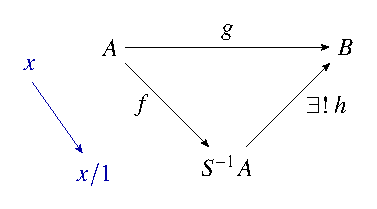
\includegraphics[width=.49\textwidth]{ca2-fig-01.pdf}
\FigureTag{CA2.1}{fig:ca-2-01}
\end{figure}
\setcounter{enumi}{3}\item For the map $f:A\to S^{-1}A$, one has:
\begin{itemize}
\item If $s\in S$, then $f(s)$ is a unit in $S^{-1}A$.
\item $f(a)=0$ implies $as=0$ for some $s\in S$.
\end{itemize}
\end{enumerate}
\end{remark}
\setcounter{example}{4}\begin{example}
If $\pp<A$ is prime, then $S=A\setminus\pp$ is multiplicatively closed. We write $S^{-1}A$ as $A_{\pp}$. The set $\mm:=\{a/s\mid a\in\pp,\ s\in S\}$ is an ideal. If $\aa\nsubseteq\mm$, there exists $b/t\in\aa$ with $b/t\notin\mm$. Hence $b\notin\pp$, so $b$ is a unit. Thus $A_{\pp}$ is a local ring.
\end{example}
\setcounter{theorem}{5}\begin{proposition}
\begin{enumerate}[label=(\roman*)]
\setcounter{enumi}{0}\item $S^{-1}$ is an exact functor.
\setcounter{enumi}{1}\item $S^{-1}(N+P)=S^{-1}N+S^{-1}P$.
\setcounter{enumi}{2}\item $S^{-1}(N\cap P)=S^{-1}N\cap S^{-1}P$.
\setcounter{enumi}{3}\item $S^{-1}(M/N)\cong S^{-1}M/S^{-1}N$.
\end{enumerate}
Here $N,P$ are $A$-submodules of $M$.
\end{proposition}
A property $P$ of an $A$-module $M$ is a \emph{local property} if
\[
(M\text{ satisfies }P)\ \Longleftrightarrow\
(M_{\pp}\text{ satisfies }P\text{ for every prime }\pp).
\]
\subsection{Extended and contracted ideals}
\setcounter{theorem}{6}\begin{proposition}
\begin{enumerate}[label=(\roman*)]
\setcounter{enumi}{0}\item Every ideal in $S^{-1}A$ is extended.
\setcounter{enumi}{1}\item For an ideal $\aa<A$,
% Source page 4
\[\aa^{ec}=\bigcup_{s\in S}(\aa:s).\]
Consequently, $\aa^e=(1)$ if $\aa$ meets $S$.
\setcounter{enumi}{2}\item $\aa\in\mathcal C$, the set of contracted ideals, if and only if no element of $S$ is a zero-divisor in $A/\aa$.
\setcounter{enumi}{3}\item Prime ideals of $S^{-1}A$ correspond to prime ideals of $A$ not meeting $S$.
\setcounter{enumi}{4}\item $S^{-1}$ commutes with finite sums, products, intersections, and radicals.
\end{enumerate}
\end{proposition}
\begin{proof}
(i) If $\bb$ is an ideal in $S^{-1}A$ and $x/s\in\bb$, then $x/1\in\bb$, so $x\in\bb^c$. Hence $x/s\in\bb^{ce}$. Since $\bb\supseteq\bb^{ce}$, we obtain $\bb=\bb^{ce}$.

(ii) One has
\[
\begin{aligned}
x\in\aa^{ec}=(S^{-1}\aa)^c
&\Longleftrightarrow x/1=b/t\quad\text{for some }b\in\aa,\ t\in S\\
&\Longleftrightarrow(xt-b)u=0\\
&\Longleftrightarrow xtu\in\aa\qquad(tu\in S)\\
&\Longleftrightarrow x\in\bigcup_{s\in S}(\aa:s).
\end{aligned}
\]
(iii) $\aa\in\mathcal C\Longleftrightarrow\aa^{ec}\subseteq\aa\Longleftrightarrow(sx\in\aa\text{ for some }s\in S\Rightarrow x\in\aa)$. In other words, we can extend $\aa$, cancel $s$, and contract. This is equivalent to no $s\in S$ being a zero-divisor in $A/\aa$.

(iv) If $\qq$ is prime in $S^{-1}A$, then $\qq^c$ is clearly prime. If $\pp$ is prime in $A$, then $A/\pp$ is an integral domain. Let $\overline S$ be the image of $S$ in $A/\pp$. Then
\[
S^{-1}A/S^{-1}\pp\cong\overline S^{-1}(A/\pp),
\]
which is either zero or contained in the field of fractions of $A/\pp$, hence an integral domain.
% Source page 5
Thus $S^{-1}\pp$ is prime or $(1)$, and $S^{-1}\pp=(1)$ if and only if $S\cap\pp\ne\varnothing$.

(v) Exercise.
\end{proof}
\setcounter{theorem}{7}\begin{corollary}
\begin{enumerate}[label=(\roman*)]
\setcounter{enumi}{0}\item If $R$ is the nilradical of $A$, then $S^{-1}R$ is the nilradical of $S^{-1}A$.
\setcounter{enumi}{1}\item If $\pp$ is prime in $A$, then primes in $A_{\pp}$ correspond to primes in $A$ contained in $\pp$.
\setcounter{enumi}{2}\item If $M$ is a finitely generated $A$-module, then $S^{-1}(\Ann M)=\Ann(S^{-1}M)$. Note that
\[
S^{-1}(\Ann(M+N))=S^{-1}(\Ann M\cap\Ann N)
=\Ann(S^{-1}(M+N)).
\]
Thus it is enough to check the result for $M$ generated by a single element.
\setcounter{enumi}{3}\item For $f:A\to B$, a prime $\pp$ is contracted if and only if $\pp^{ec}=\pp$.
\end{enumerate}
\end{corollary}
% BLOG-CONTENT-END
\end{document}
